\newpage
\section{RESEARCH METHODOLOGY} 
\subsection{Introduction}
The basic structure for this research work is presented in this section. This section presents the research design, along with conceptual framework, detailing how the research work has been conducted to achieve the research objectives. Thus, this section contains the details of the research design, conceptual framework, sources of data, tools of analysis, along with operational definition of the variables used in this research.  
\vspace{-5mm}
\subsection{Research Design}
To achieve the objectives of this thesis, the research will employ descriptive and explanatory research design. The first objective, which is to analyze low local levels of Nepal differ in fiscal, economic, and electoral sense will be conducted through descriptive design. The second objective, to gauge the impact of electorate on fiscal decision making of elected officials, will be carried out through explanatory research design. The study will use the data collected from the first local level election in 2017, the subsequent fiscal and economic data of local levels from variety of sources, and the census of 2021. Since the data collected is of all 753 local level of Nepal over the period of five years, the study will have a panel data, which will be changed to cross-sectional data. 
\vspace{-3mm}
\subsection{Conceptual Framework}
In empirical research, a conceptual framework serves as a critical blueprint that outlines the key variables and their interrelationships. It provides a structured approach to understanding how different factors influence the phenomenon under investigation. The following diagram shows how electoral competition, through electoral accountability, influences the fiscal and economic disciplines of the local level of Nepal. The conceptual framework, as shown in the figure \ref{Conceptual Framework}, shows the overall process of our research design.
\newpage
\begin{figure}[h]
\centering
\hspace{-1.2cm}
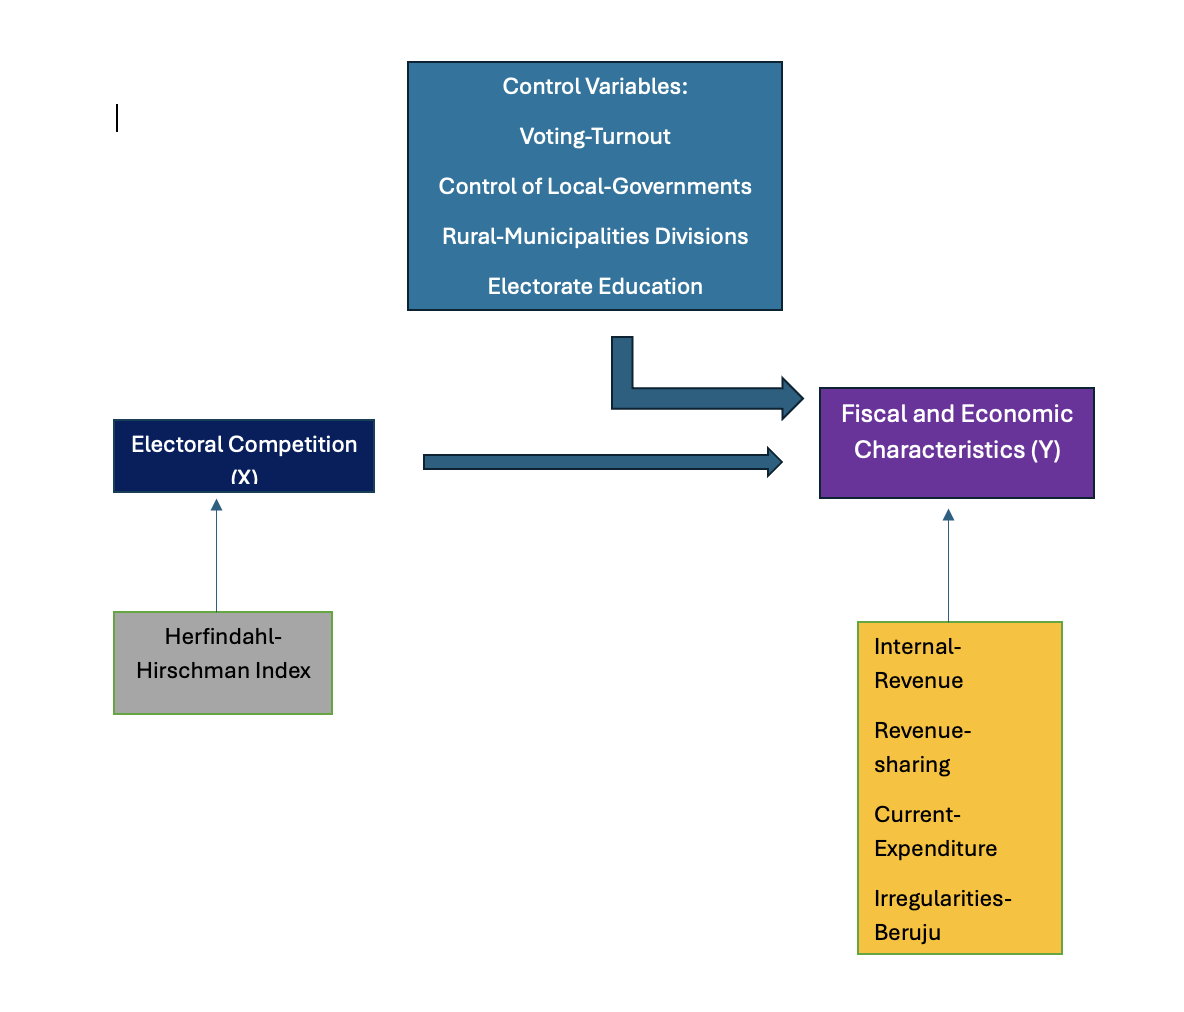
\includegraphics[width = 170mm, scale = 0.4]{figure/Conframe.png}
\caption{Conceptual Framework of the study}
\label{Conceptual Framework}
\end{figure}
\subsection{Sources of data}
Data have been collected from bevy of sources for this empirical study. The data related to election which are used to construct Herfindahl-Hirschman index and Voting-Turnout variables, were collected from the Election Commission of Nepal website\footnote{election.gov.np} and official publications of the Election Commission. The data on the status of local levels were collected from the Ministry of Federal Affairs and General Administration\footnote{mofaga.gov.np}.  \\
The data on the composition of the local governments were taken from the respective local government websites as well as from the Election Commission, whereas the data on the education status of the local level were taken from the census result of 2021 provided by the CBS. For the fiscal and economic characteristics, including, data on internal revenue each year, income from revenue sharing, current expenditure, and irregularities/Beruju, the data were taken from the annual published report of AG and cross verified through matching it with the respective local levels.
\vspace{-5mm}
\subsection{Operational Definitions of Variables}
The study uses the following variables in the descriptive and explanatory analysis. The Acronym provided here will be used while specifying the model too.\\
\textit{\underline{Independent Variables:}}\\
\textbf{Herfindahl-Hirschman Index:} HHI is a measure of electoral competition and concentration. It quantifies the level of concentration among mayoral candidates in the 2017 election of Nepal, indicating how evenly or unevenly votes were distributed among them. The score theoretically ranges from 0 to 1, where score closer to 0 indicates the more competitive election while the score closer to 1 indicates more uncompetitive election, where a few candidates dominate the vote share. To make the calculation simple, we only take top four vote receivers, and sum others into another group, where applicable as most constituency did not have more than five candidates.The HHI in our study has been calculated following these steps:\\
\begin{enumerate}[label=\roman*.]  
     \item Obtaining the share of vote of each candidates in the election, thus, dividing the vote received by each candidates by the total vote.
    \item The next step is squaring the vote share of each candidates.
    \item The final step is to sum the squared share of all the candidates of the election. Thus, it could be written as the following formula:
\end{enumerate}
\[HHI =\sum_{i-1}^{n}(s_i)^2\]\\ 
where \(s_i \) is the vote share of the mayoral candidate \( i \), and \( n \) is the total number of candidates.\\
\textit{\underline{Control Variables:}}\\
\textbf{Voting-Turnout:} Vote-Turnout is, as the name implies, the percentage of total electorate that voted in the election. Thus, the percentage theoretically ranges between 0 to 100, but seldom is 0. \\
\textbf{Control of Local-Governments:} Divided-Control, is a dummy variable which indicates if the mayors and deputy mayors are of the same party with the majority of ward members. Thus, it takes a value of 0 if the mayor and deputy mayor are of the same party with the majority of ward members, thus no divided control, and 1 when mayor and deputy mayor are not of the same party, or when they are of the same party but they do not have the majority of ward members of the same party.\\
\textbf{Rural-Municipalities category:} DummyRM, is a dummy variable which indicates if the local jurisdiction is a Rural-Municipality. If the local government is a Rural-Municipality, it is 1 and if it is not, the value is 0.\\
\textbf{Electorate Education:} Highedu, is a variable that measures the percentage of people of the local area who have completed intermediate level or more. The data is a courtesy of CBS, which is based on the 2021 census. Since the education data does not change fast, this study takes the data of 2021 to be applicable to years from 2019 to 2022. \\
\textit{\underline{Dependent Variables:}}\\
\textbf{Internal-Revenue:} Intrevtot, is a variable that measures the internal income generated by the local level divided by the total revenue of that local level. Thus, this variable gives us what percentage of total revenue of that local level was generated internally by the concerned local level. The study expects that independent variable,HHI, to have negative association with this variable as when HHI value increases, it means the decrease in electoral competition and through less accountability, the elected officials will not do their utmost to improve internal income \\
\textbf{Revenue-Sharing:} Revshrtot, is a variable that calculates the income earned by the local levels as a fraction of their total revenue, from sharing the revenue with the provincial and central government. The study expects negative association with HHI for the same reason as mentioned in Internal-Revenue variable section.\\
\textbf{Current Expenditure:} Curexp variable is the fraction of the current expenditure of the local level to its total expenditure. The study expects positive association with HHI as increase in HHI means decrease in electoral competition, which could weaken accountability and motivate the elected officials to spend more on current expenditures.\\
\textbf{Irregularities-Beruju:} Berujupc variable measures the `Beruju' of each local level in a per capita basis. Raw comparison of it would not be wise as there are local levels with different stratum of expenditures and thus, per capita technique is applied. This study expects a positive association with HHI for the same reason as mentioned in Current Expenditure variable.
\vspace{-3mm}
\subsection{Tools of analysis}
\subsubsection{Descriptive Analysis}
This study performs the descriptive analysis of the variable used in the model using statistical tools such as mean, median, and standard deviation to give context to the variables. Thus, in the next section, this study would provide the descriptive statistics of variables like HerfindahI-Hirschman Index, Vote-Turnout, Education level, Internal income of local governments among other variables.
\subsubsection{Explanatory Analysis}
The examination of relationship between electoral competition, as given by HHI, with the variables of fiscal and economic discipline will be carried out. As we have the panel data, and the independent variable and control variables are all time-invariant, while the dependent variables of fiscal and economic decisions are all time variant, \citeA{Wooldridge2009} and \citeA{Wooldridge2010} states that neither fixed effect regression model nor random effect model could be used as key regressors are time-invariant. Thus, this study merges and averages the dependent variables and uses OLS estimator. While panel structure would have allowed for the analysis of effects across multiple years, this study intends to capture broad, long-term effect and using cross-sectional data is valid for it.
\vspace{-4mm}
\subsubsection{Model Specification}
This study will be using OLS linear regression and pooled cross sectional regression to investigate the relationship between the independent and dependent variables. The first empirical model can be written as follows:
\begin{equation}
FiscalDiscipline_i = \beta_0 + \beta_1 HHI_i + \beta_2 VoterTurnout_i + \beta_3 Divcontrol_i+  \beta_4 highedu _i+ \beta_5 DumRM_i + \epsilon
\end{equation}
Where:\\
- \(FiscalDiscipline\) refers to the fiscal discipline variables (Intrevtot, Revshrtot, Curexp, and Berujupc will be used ).\\
- \(HHI\) (Herfindahl-Hirschman Index) measures political concentration at mayoral level.\\
- \(VoterTurnout\) represents the voting percentage.\\
- \(Divcontrol\) is a dummy variable indicating whether the control of the jurisdiction is divided or not.\\
- \(highedu\) refers to the percentage of highly educated(intermediate or more) individuals.\\
- \(DumRM\) is a dummy variable indicating rural or municipal areas.\\
- \(\beta_0\) is the intercept.\\
- \(\epsilon\) is the error term.\\
Each coefficient \(\beta_1, \beta_2, \beta_3, \beta_4, \beta_5\) will represent the estimated effect of the corresponding independent variable on the variables of fiscal discipline.\\
Since the cross sectional regression merges the panel observations, without taking account of time variation, and would not account for autocorrelations in the residuals, this study also runs a pooled regression with the following equation:
\begin{align}
Y_{it} & = \beta_0 + \beta_1 \text{HHI}_i + \beta_2 \text{VoterTurnout}_i + \beta_3 \text{HighEduRate}_i \nonumber \\ &\quad + \beta_4 \text{DumRM}_i + \beta_5 \text{DivControl}_i + \gamma_t D_t + \epsilon_{it} 
\end{align}
Where:\\
-\(Y_{it}\) = Dependent variable (Intrevtot, Revshrtot, Curexp, and Berujupc of local level  i at time  t.\\
-\(HHI_{i}\), \(VoterTurnout_{i}\), \(HighEduRate_{i}\), \(DumRM_{i}\), \(DivControl_{i}\) = Time-invariant independent variables, same as in equation (1)\\
-\(D_t\) = Dummy variables for the years 2019, 2020, and 2021 (to control for time effects).\\
-\(\gamma_t \)= Coefficients for the time dummies.\\
-\(\epsilon_{it}\) = Error term.

